% questions.tex —— 1987 年·全国卷·文科 · 题目内容片段（无答案）
% 由 tools/generate_projects.py 依来源总账自 1987/1987_数学真题_全国文_试题.md 生成，勿手改（改源 MD 后重跑）


\gkpart{文科数学}

\begin{gktip}
\textbf{来源说明}：本题面依据固定源 PDF《1987 普通高等学校招生考试（全国卷文）》逐题转录。固定源共 1 页 A3 横向扫描，原卷页码 31；第 1—8 题为选择题，第 9—16 题为填空题，第 17—22 题为解答题。固定源不含答案或解析页，答案和解析依据题面独立复算。

\textbf{图形说明}：第 5、8、18 题的图形依据固定源关系重绘为 TikZ 矢量图。第 17、22 题按完整题面保留两个可能的结果。
\end{gktip}

\begin{question}
\gkti{1}设 $S\text{、}T$ 是两个非空集合，且 $S\nsubseteq T$，$T\nsubseteq S$，令 $X=S\cap T$，那么 $S\cup X$ 等于\mbox{（　　）}

（A）$X$　　（B）$T$　　（C）$\varnothing$　　（D）$S$

\end{question}
\begin{question}
\gkti{2}设椭圆方程为

\nopagebreak[4]
\[
\frac{x^2}{a^2}+\frac{y^2}{b^2}=1\qquad(a>b>0),
\]

令 $c=\sqrt{a^2-b^2}$，那么它的准线方程为\mbox{（　　）}

（A）$y=\pm\dfrac{a^2}{c}$　　（B）$y=\pm\dfrac{b^2}{c}$

（C）$x=\pm\dfrac{a^2}{c}$　　（D）$x=\pm\dfrac{b^2}{c}$

\end{question}
\begin{question}
\gkti{3}设

\nopagebreak[4]
\[
\log_3 4\cdot\log_4 8\cdot\log_8m=\log_4 16,
\]

那么 $m$ 等于\mbox{（　　）}

（A）$\dfrac92$　　（B）$9$　　（C）$18$　　（D）$27$

\end{question}
\begin{question}
\gkti{4}复数 $\sin40^\circ-i\cos40^\circ$ 的辐角为\mbox{（　　）}

（A）$40^\circ$　　（B）$140^\circ$　　（C）$220^\circ$　　（D）$310^\circ$

\Needspace{0.4\textheight}
\end{question}
\begin{question}
\gkti{5}二次函数 $y=f(x)$ 的图象如图所示，那么此函数为\mbox{（　　）}
\nopagebreak[4]
\begin{center}% 1987 年全国卷文科第五题：二次函数图象
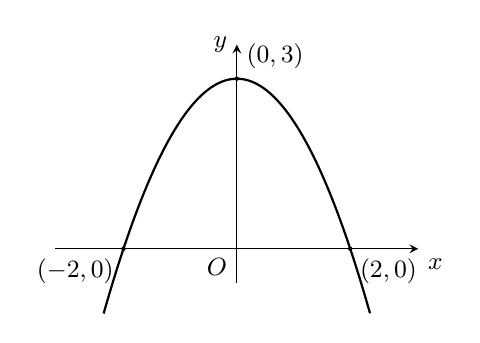
\begin{tikzpicture}[scale=0.72,>=stealth,font=\small]
  \draw[->] (-3.2,0)--(3.2,0) node[below right] {$x$};
  \draw[->] (0,-0.6)--(0,3.6) node[left] {$y$};
  \draw[thick,domain=-2.35:2.35,samples=80]
    plot (\x,{3-0.75*\x*\x});
  \fill (-2,0) circle (1.1pt) node[below left] {$(-2,0)$};
  \fill (2,0) circle (1.1pt) node[below right] {$(2,0)$};
  \fill (0,3) circle (1.1pt) node[above right] {$(0,3)$};
  \node[below left] at (0,0) {$O$};
\end{tikzpicture}
\end{center}
\nopagebreak[4]
（A）$y=x^2-4$　　（B）$y=4-x^2$

（C）$y=\dfrac34(4-x^2)$　　（D）$y=\dfrac34(2-x^2)$

\end{question}
\begin{question}
\gkti{6}在区间 $(-\infty,0)$ 上为增函数的是\mbox{（　　）}

（A）$y=-\log_{\frac12}(-x)$　　（B）$y=\dfrac{x}{1-x}$

（C）$y=-(x+1)^2$　　（D）$y=1+x^2$

\end{question}
\begin{question}
\gkti{7}已知平面上一点 $P$ 在原坐标系中的坐标为 $(0,m)$（$m\ne0$），而在平移后所得到的新坐标系中的坐标为 $(m,0)$，那么新坐标系的原点 $O'$ 在原坐标系中的坐标为\mbox{（　　）}

（A）$(-m,m)$　　（B）$(m,-m)$　　（C）$(m,m)$　　（D）$(-m,-m)$

\Needspace{0.4\textheight}
\end{question}
\begin{question}
\gkti{8}要得到函数

\nopagebreak[4]
\[
y=\sin\left(2x-\frac\pi3\right)
\]

的图象，只需将函数 $y=\sin2x$ 的图象（如图）\mbox{（　　）}
\nopagebreak[4]
\begin{center}% 1987 年全国卷文科第八题：y=sin 2x 的示意图
\begin{tikzpicture}[scale=0.72,>=stealth,font=\small]
  \draw[->] (-1.9,0)--(3.55,0) node[below right] {$x$};
  \draw[->] (0,-1.45)--(0,1.55) node[left] {$y$};
  \draw[thick,domain=-1.75:3.25,samples=160,smooth]
    plot (\x,{sin(deg(2*\x))});
  \node[below] at (-1.57,0) {$-\dfrac\pi2$};
  \node[below right] at (0.05,0) {$O$};
  \node[below] at (1.57,0) {$\dfrac\pi2$};
  \node[below] at (3.14,0) {$\pi$};
  \node[left] at (0,1) {$1$};
  \node[left] at (0,-1) {$-1$};
\end{tikzpicture}
\end{center}
\nopagebreak[4]
（A）向左平行移动 $\dfrac\pi3$　　（B）向右平行移动 $\dfrac\pi3$

（C）向左平行移动 $\dfrac\pi6$　　（D）向右平行移动 $\dfrac\pi6$

\end{question}
\begin{question}
\gkti{9}求函数

\nopagebreak[4]
\[
y=\sin^2 2x
\]

的周期。

\end{question}
\begin{question}
\gkti{10}已知方程

\nopagebreak[4]
\[
\frac{x^2}{2+\lambda}-\frac{y^2}{1+\lambda}=1
\]

表示双曲线，求 $\lambda$ 的范围。

\end{question}
\begin{question}
\gkti{11}若 $(1+x)^n$ 的展开式中，$x^3$ 的系数等于 $x$ 的系数的 7 倍，求 $n$。

\end{question}
\begin{question}
\gkti{12}求极限

\nopagebreak[4]
\[
\lim_{n\to\infty}\left(\frac1{n^2}+\frac2{n^2}+\frac3{n^2}+\cdots+\frac{2n}{n^2}\right).
\]

\end{question}
\begin{question}
\gkti{13}由数字 $1\text{、}2\text{、}3\text{、}4\text{、}5$ 组成没有重复数字且数字 1 与 2 不相邻的五位数，求这种五位数的个数。

\end{question}
\begin{question}
\gkti{14}求函数

\nopagebreak[4]
\[
y=\log_2(1+2x-3x^2)
\]

的定义域。

\end{question}
\begin{question}
\gkti{15}圆锥底面积为 $3\pi$，母线与底面所成的角为 $60^\circ$，求它的体积。

\end{question}
\begin{question}
\gkti{16}发电厂发出的电是三相交流电，它的三根导线上的电流强度分别是时间 $t$ 的函数：

\nopagebreak[4]
\[
I_A=I\sin\omega t,\qquad
I_B=I\sin(\omega t+120^\circ),\qquad
I_C=I\sin(\omega t+240^\circ).
\]

求 $I_A+I_B+I_C$ 的值。

\end{question}
\begin{question}
\gkti{17}在复平面内，已知等边三角形的两个顶点表示的复数分别为

\nopagebreak[4]
\[
2,\qquad \frac12+\frac{\sqrt3}{2}i,
\]

求第三个顶点表示的复数。

\Needspace{0.4\textheight}
\end{question}
\begin{question}
\gkti{18}如图，三棱锥 $P-ABC$ 中，已知 $PA\perp BC$，$PA=BC=L$，$PA\text{、}BC$ 的公垂线 $ED=h$。求证：三棱锥 $P-ABC$ 的体积

\nopagebreak[4]
\[
V=\frac16L^2h.
\]
\nopagebreak[4]
\begin{center}% 1987 年全国卷文科第十八题：三棱锥 P-ABC 与公垂线 ED
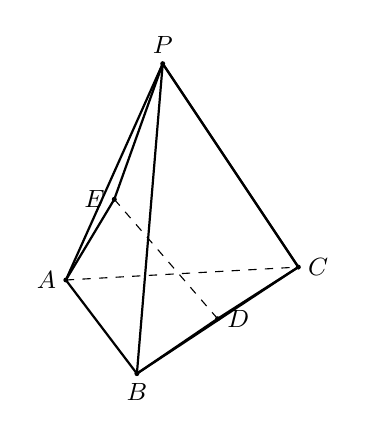
\begin{tikzpicture}[scale=0.82,>=stealth,font=\small]
  \coordinate (P) at (1.6,3.8);
  \coordinate (A) at (0.1,0.45);
  \coordinate (B) at (1.2,-1.0);
  \coordinate (C) at (3.7,0.65);
  \coordinate (E) at (0.85,1.7);
  \coordinate (D) at (2.45,-0.15);
  \draw[thick] (P)--(A)--(B)--(C)--cycle;
  \draw[thick] (P)--(B) (P)--(C);
  \draw[dashed] (A)--(C);
  \draw[dashed] (E)--(D);
  \draw[thick] (P)--(E) (E)--(A);
  \draw[thick] (B)--(D)--(C);
  \fill (P) circle (1.1pt) node[above] {$P$};
  \fill (A) circle (1.1pt) node[left] {$A$};
  \fill (B) circle (1.1pt) node[below] {$B$};
  \fill (C) circle (1.1pt) node[right] {$C$};
  \fill (E) circle (1.1pt) node[left] {$E$};
  \fill (D) circle (1.1pt) node[right] {$D$};
\end{tikzpicture}
\end{center}
\nopagebreak[4]
\end{question}
\begin{question}
\gkti{19}设对所有实数 $x$，不等式

\nopagebreak[4]
\[
x^2\log_2\frac{4(a+1)}a
+2x\log_2\frac{2a}{a+1}
+\log_2\frac{(a+1)^2}{4a^2}>0
\]

恒成立，求 $a$ 的取值范围。

\end{question}
\begin{question}
\gkti{20}设复数 $z_1$ 和 $z_2$ 满足关系式

\nopagebreak[4]
\[
z_1\overline{z_2}+\overline A z_1+A\overline{z_2}=0,
\]

其中 $A$ 为不等于 0 的复数。证明：

\Needspace{5\baselineskip}
（1）　

\nopagebreak[4]
\[
|z_1+A||z_2+A|=|A|^2\text{；}
\]

\Needspace{5\baselineskip}
（2）　

\nopagebreak[4]
\[
\frac{z_1+A}{z_2+A}
=\frac{\overline{z_1+A}}{\overline{z_2+A}}.
\]

\Needspace{12\baselineskip}

\end{question}
\begin{question}
\gkti{21}设数列 $a_1,a_2,\ldots,a_n,\ldots$ 的前 $n$ 项的和 $S_n$ 与 $a_n$ 满足

\nopagebreak[4]
\[
S_n=ka_n+1
\]

（其中 $k$ 是与 $n$ 无关的常数，且 $k\ne1$）。

（1） 试写出用 $n\text{、}k$ 表示的 $a_n$ 的表达式；

\Needspace{5\baselineskip}
（2） 若

\nopagebreak[4]
\[
\lim_{n\to\infty}S_n=1,
\]

求 $k$ 的取值范围。

\end{question}
\begin{question}
\gkti{22}正方形 $ABCD$ 在直角坐标平面内，已知其一条边 $AB$ 在直线 $y=x+4$ 上，$C\text{、}D$ 在抛物线 $x=y^2$ 上，求正方形 $ABCD$ 的面积。

\end{question}